\documentclass{beamer}
\usepackage{../../typesetting/styles/slide-zh}
\usepackage{bookmark}

\title{\LARGE{周报}}
\subtitle{}
\author{}
\date{2025-04-21}

\begin{document}

% Title frame
\begin{frame}
  \titlepage
\end{frame}

% Outline frame
\begin{frame}{大纲}
  \tableofcontents
\end{frame}

\section{论文修改和查重}
\begin{frame}{论文写作进展与查重}
  \begin{block}{本周重点}
    \begin{itemize}
      \item 完成论文图表的\textcolor{blue}{尺寸调整}与\textcolor{blue}{排版优化}
      \item 提升论文内容的\textcolor{blue}{学术表达}与逻辑性
      \item 优化所有图片和表格的版面显示
      \item 精炼部分段落,提升表达准确性
      \item 进行\textcolor{blue}{重复率检测},\textcolor{red}{相似度指数仅为10\%},符合投稿要求
    \end{itemize}
  \end{block}
  \begin{center}
    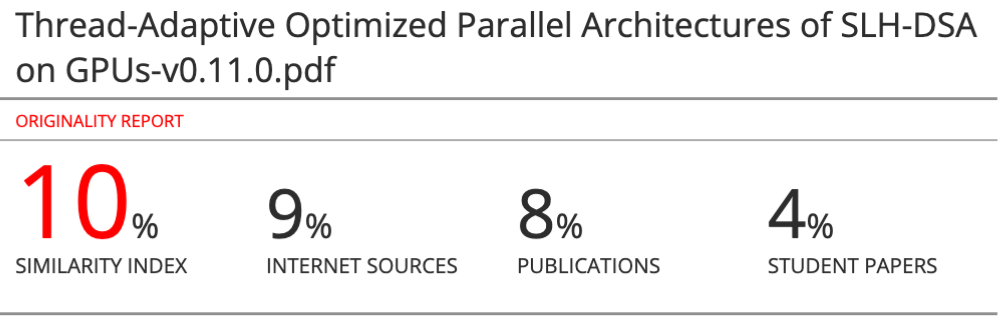
\includegraphics[width=0.45\textwidth]{fig/reptition.png}\\
    \footnotesize{论文查重结果}
  \end{center}
\end{frame}

\section{期刊选择}
\begin{frame}{期刊选择与调研}
  \begin{block}{调研与对比}
    检索\textcolor{red}{IEEE Transactions}系列期刊,查阅投稿指南,关注稿件格式、审稿周期、版面费、录用率等信息。\textcolor{red}{大部分顶级Transactions期刊不接受Letter/Brief类论文},因此\textcolor{red}{TCAS-II}更适合本次简报类稿件。下表为主要目标期刊对比:
    \vspace{1ex}
    \begin{center}
      \scriptsize
      \begin{tabular}{lcccc}
        \toprule
        期刊名称 & 分区 & IF值 & 审稿周期(月) & 年文章数 \\
        \midrule
        \textcolor{red}{\textbf{IEEE Trans. Circuits Syst. II Express Briefs}} & \textcolor{red}{2区} & \textcolor{red}{4.4} & \textcolor{red}{3} & \textcolor{red}{1050} \\
        IEEE Communications Letters  & 3区 & 4.1 & 3 & 680 \\
        IEEE Signal Processing Letters  & 3区 & 3.2 & 3 & 366 \\
        \bottomrule
      \end{tabular}
    \end{center}
    \vspace{1ex}
    \textcolor{red}{TCAS-II}已发表相关GPU加速AES文章\cite{Lee2022Jeong},优先选择为投稿目标。
  \end{block}
\end{frame}

\begin{frame}{老师评语}
  \begin{alertblock}{注意论文中的实验结果图全是表格,可以多样化,特别是对比图
    trans论文最注重用图表来表述论文核心}
    替换部分表格为图表,添加核心性能对比图
  \end{alertblock}
  \begin{alertblock}{可以投第一个trans,trans论文在业内还是非常认可的(不管几区都认为是top期刊)}
    好的
  \end{alertblock}
  \begin{block}{下周计划}
    \begin{itemize}
      \item \textcolor{blue}{对论文修改}
      \item \textcolor{blue}{准备期刊投稿所需材料}
    \end{itemize}
  \end{block}
\end{frame}

\begin{frame}
  \frametitle{参考文献}
  \bibliographystyle{alpha}
  \bibliography{../../paper}
\end{frame}

\end{document}
